\begin{table}
\begin{minipage}[t]{0.45\linewidth}
\setlength{\tabcolsep}{4pt}
% \begin{adjustbox}{max width=\linewidth}
\scriptsize
\caption{Example of tool manipulation errors. Errors are highlighted in red.}\label{tab:typical_errors}
\begin{tabular}{cl}
\toprule
\textbf{Goal}           & \begin{tabular}[c]{@{}l@{}}\# To move the robot to position (x, y)\\ robot.move\_to(x, y)\\ \# To raise the arm by a given height\\ robot.raise\_arm(height)\\ Task: how to move a robot to (20, 30)?\end{tabular} \\
\cmidrule(lr){1-2}
\textbf{Expected results} & robot.move\_to(20, 30)                                                                                                                                                                                                                   \\
\midrule
\textbf{Wrong API}        & robot.{\color{red}\textbf{raise\_arm}}(20)                                                                                                                                                                                                                     \\
\cmidrule(lr){1-2}
\textbf{Wrong Arguments}      & robot.move\_to({\color{red}\textbf{30, 20}})                                                                                                                                                                                                                  \\
\cmidrule(lr){1-2}
\textbf{Non-executable}        & \begin{tabular}[c]{@{}l@{}} {\color{red}\textbf{You can create a robot with}} \\ {\color{red}\textbf{robot = Robot()}}\\ {\color{red}\textbf{and move it to the target location by}} \\ robot.move\_to(20, 30)\end{tabular}                                                  \\
\bottomrule
\end{tabular}
% \end{adjustbox}
\end{minipage}
\hspace{1em}
\begin{minipage}[t]{0.525\linewidth}
\setlength{\tabcolsep}{-1pt}

\captionof{figure}{Without API documentation exposure during inference, closed LLMs attain high accuracy in selecting APIs (left), implying potential example usage exposure during training. Hand-picked oracle one-shot demonstration improves success rate over zero-shot on the OpenWeather (right), showing the roofline impact of in-context demonstrations.}\label{fig:obsv_123}
\vspace{-3pt}
\begin{tabular}{c c}
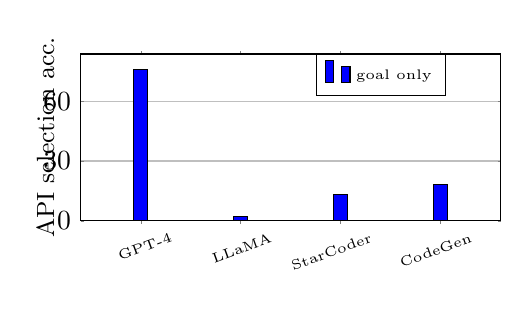
\begin{tikzpicture}[]
    \begin{axis}[
        ybar=0.0cm,
        % Size
        width=0.57\linewidth,
        height=3.7cm,
        bar width=5pt,
        enlarge x limits=0.2,
        ymajorgrids,
        % Axes
        ylabel={API selection acc.},
        ymin=0,
        xtick=data,
        ytick={0, 30, 60, 90},
        x tick label style={xshift=3ex,rotate=20,anchor=east,yshift=-4pt,font=\tiny},
        y label style={yshift=-2.5ex, font=\small},
        symbolic x coords = {GPT-4, LLaMA, StarCoder, CodeGen},
        tickwidth         = 1pt,
        % Legend
        legend style={
            at={(0.715,1)},
            anchor=north,
            legend columns=1,
            font=\tiny,
            /tikz/every even column/.append style={column sep=0.cm, row sep=-2pt},
        },
        ]
        
        % goal only, with "To achieve this request, utilize Curl to make a GET request and call the OpenWeather API. (Answer in code only)"
        \addplot[black, fill=blue] coordinates { 
            (GPT-4, 76)
            % (LLaMA, 11)
            % (NeoX-20b, 28)
            (LLaMA, 2)
            (CodeGen, 18)
            (StarCoder, 13)
        };

        % % API doc + goal, with "(Answer in code only)"
        % \addplot[black, fill=red, postaction={pattern=north east lines}] coordinates {
        %     (GPT-4, 99)
        %     % (LLaMA, 14)
        %     % (NeoX-20b, 68)
        %     % (CodeGen, 59)
        %     (LLaMA, 33)
        %     (StarCoder, 3)
        % };
                    
        % Some legend hacks
        \legend{}
        \addlegendimage{black, fill=blue}
        \addlegendentry{goal only}
        % \addlegendimage{black, fill=red, postaction={pattern=north east lines}}
        % \addlegendentry{API doc + goal}
    \end{axis}
\end{tikzpicture} &
\begin{tikzpicture}[]
    \begin{axis}[
        ybar=0.0cm,
        % ybar interval=0.3,
        enlarge x limits=0.2,
        % enlarge y limits=0.2,
        % Size
        width=0.57\linewidth,
        height=3.7cm,
        % bar width=6pt,
        bar width=5,
        ymajorgrids,
        % Axes
        ylabel={Success rate},
        ymin=0,
        xtick=data,
        ytick={0, 20, 40, 60, 80},
        % ytick={0, 30, 60, 90},
        x tick label style={xshift=3ex,rotate=20,anchor=east,yshift=-4pt,font=\tiny},
        y label style={yshift=-3ex, font=\small},
        % symbolic x coords = {GPT-4, LLaMA-30b, NeoX-20b, CodeGen-mono-16b},
        symbolic x coords = {GPT-4, LLaMA, StarCoder, CodeGen},
        tickwidth         = 1pt,
        % Legend
        legend style={
            at={(0.715,1)},
            anchor=north,
            legend columns=1,
            font=\tiny,
            /tikz/every even column/.append style={column sep=0.cm, row sep=-6pt},
        },
        ]
        
        % zero-shot, with API doc, without "(Answer in code only)"
        \addplot[black, fill=blue] coordinates { 
            (GPT-4, 81)
            (LLaMA, 39)
            % (NeoX-20b, 18)
            (CodeGen, 7)
            (StarCoder, 32)
        };

        % oracle one-shot, with API doc, without "(Answer in code only)"
        \addplot[black, fill=red, postaction={pattern=north east lines}] coordinates {
            (GPT-4, 89)
            (LLaMA, 62) % <-- manualy reduced to 57 for better visuaization
            % (NeoX-20b, 38)
            (CodeGen, 52)
            (StarCoder, 67)
        };
                    
        % Some legend hacks
        \legend{,}
        \addlegendimage{black, fill=blue}
        \addlegendentry{zero-shot}
        \addlegendimage{black, fill=red, postaction={pattern=north east lines}}
        \addlegendentry{one-shot}
    \end{axis}
\end{tikzpicture}
\end{tabular}
\end{minipage}

% \vspace{-20pt}
\end{table}


\begin{wraptable}[9]{r}{0.55\textwidth}
 \vspace{-1.1em}
\captionof{table}{Categorized typical tool manipulation error types on a weather query tool.}
\label{tab:error_breakdown}
\small
 \vspace{-0.45em}
\begin{tabular}{@{}cc@{\hskip 0.5em}c@{\hskip 0.5em}c@{\hskip 0.5em}c}
\toprule
\multicolumn{1}{l}{} & GPT-4 & LLaMA & StarCoder & CodeGen \\
\cmidrule(lr){2-5}
% \midrule
Failure rate       & 19\% & 61\%  & 68\%  & 93\%            \\
\midrule
API selection      & 0\%  & 22\%  & 22\%  & 30\%             \\
Args. populating   & 14\% & 32\%  & 23\%  & 63\%             \\
Non-executable     & 5\%  & 7\%   & 23\%  & 0\%	           \\
\bottomrule
\end{tabular}
\end{wraptable}
To demystify key challenges, we study the behaviors of open-source LLMs in tool manipulation. By analyzing common mistakes in a weather query task,
% which requires only a single API call to accomplish each task, 
we discover three challenges to attain strong tool manipulation capabilities. As shown in~\Cref{tab:typical_errors}, we observe that open-source LLMs often 
% 1) have difficulties in selecting APIs for certain goals,
% 2) struggle with populating API arguments,
% and 3) produce generations that are not directly executable
face difficulty in (1) API selection, (2) API argument population, and (3) generating legitimate and executable code
\footnote{If a failure case has multiple errors, we categorize it by the first triggered category in the following order: non-executable generation, wrong API selection, wrong argument populating}. 
These insights are described in detail in this section and inspire the techniques to alleviate the challenges in~\Cref{sec:techniques}. 
% \comment{Jian: let's mention openweather API here? since all 3 insights are from it}
% in~\Cref{sec:techniques}. 

% In this section, we conduct several preliminary experiments on a relatively simple task: retrieve weather information from the OpenWeather\footnote{https://openweathermap.org/api} website via REST API, using natrual language command. This task contains 9 different API functions in total, but to accomplish each test request, only one API function call is needed. The detail of this task is described in section \ref{sec:benchmarks}.

\paragraph{Difficulty in API selection}
% \begin{wrapfigure}[10]{r}{4.2cm}
% \vspace{-12pt}
% \caption{Internalized knowledge improves API selection on the OpenWeather.}\label{fig:obsv_3}
% 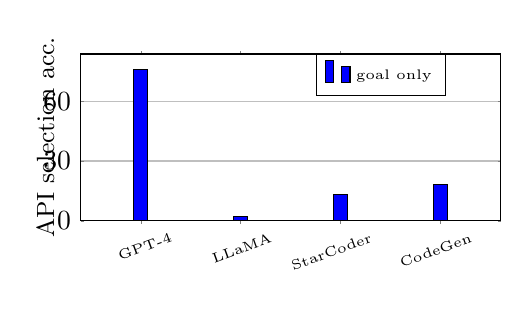
\begin{tikzpicture}[]
    \begin{axis}[
        ybar=0.0cm,
        % Size
        width=0.57\linewidth,
        height=3.7cm,
        bar width=5pt,
        enlarge x limits=0.2,
        ymajorgrids,
        % Axes
        ylabel={API selection acc.},
        ymin=0,
        xtick=data,
        ytick={0, 30, 60, 90},
        x tick label style={xshift=3ex,rotate=20,anchor=east,yshift=-4pt,font=\tiny},
        y label style={yshift=-2.5ex, font=\small},
        symbolic x coords = {GPT-4, LLaMA, StarCoder, CodeGen},
        tickwidth         = 1pt,
        % Legend
        legend style={
            at={(0.715,1)},
            anchor=north,
            legend columns=1,
            font=\tiny,
            /tikz/every even column/.append style={column sep=0.cm, row sep=-2pt},
        },
        ]
        
        % goal only, with "To achieve this request, utilize Curl to make a GET request and call the OpenWeather API. (Answer in code only)"
        \addplot[black, fill=blue] coordinates { 
            (GPT-4, 76)
            % (LLaMA, 11)
            % (NeoX-20b, 28)
            (LLaMA, 2)
            (CodeGen, 18)
            (StarCoder, 13)
        };

        % % API doc + goal, with "(Answer in code only)"
        % \addplot[black, fill=red, postaction={pattern=north east lines}] coordinates {
        %     (GPT-4, 99)
        %     % (LLaMA, 14)
        %     % (NeoX-20b, 68)
        %     % (CodeGen, 59)
        %     (LLaMA, 33)
        %     (StarCoder, 3)
        % };
                    
        % Some legend hacks
        \legend{}
        \addlegendimage{black, fill=blue}
        \addlegendentry{goal only}
        % \addlegendimage{black, fill=red, postaction={pattern=north east lines}}
        % \addlegendentry{API doc + goal}
    \end{axis}
\end{tikzpicture}
% \end{wrapfigure} 
% Comparing to code-only generation and argument filling, choosing the right API to use could requires substantially more world knowledge. 
% For instance, triggering the REST API call requires an action generator knowing the base url address of the weather query service. 
We observe that API selection failures often involve using incorrect APIs and even hallucinating non-existent API names.
To quantitatively understand the intrinsic capability in API selection, we compare open-source LLMs to GPT-4 without providing any documentation or in-context demonstrations during inference. The results, as shown in Figure \ref{fig:obsv_123} for the weather query tool OpenWeather, reveal that GPT-4 can choose the right API without additional information beyond the goal, while open-source models struggle. Such capability disparity entails that \emph{closed LLMs potentially internalize knowledge of API usage during training}.
% and help the model to better accomplish tasks in practice when the API functions are provided in prompt. 
% Comparing to code-only generation and argument filling, choosing the right API to use could requires substantially more world knowledge. 

\paragraph{Confusion in populating arguments}
% \begin{wrapfigure}[11]{r}{4.2cm}
% \vspace{-12pt}
% \caption{Oracle one-shot improves success rate over zero-shot on the OpenWeather.}\label{fig:obsv_1}
% \begin{tikzpicture}[]
    \begin{axis}[
        ybar=0.0cm,
        % ybar interval=0.3,
        enlarge x limits=0.2,
        % enlarge y limits=0.2,
        % Size
        width=0.57\linewidth,
        height=3.7cm,
        % bar width=6pt,
        bar width=5,
        ymajorgrids,
        % Axes
        ylabel={Success rate},
        ymin=0,
        xtick=data,
        ytick={0, 20, 40, 60, 80},
        % ytick={0, 30, 60, 90},
        x tick label style={xshift=3ex,rotate=20,anchor=east,yshift=-4pt,font=\tiny},
        y label style={yshift=-3ex, font=\small},
        % symbolic x coords = {GPT-4, LLaMA-30b, NeoX-20b, CodeGen-mono-16b},
        symbolic x coords = {GPT-4, LLaMA, StarCoder, CodeGen},
        tickwidth         = 1pt,
        % Legend
        legend style={
            at={(0.715,1)},
            anchor=north,
            legend columns=1,
            font=\tiny,
            /tikz/every even column/.append style={column sep=0.cm, row sep=-6pt},
        },
        ]
        
        % zero-shot, with API doc, without "(Answer in code only)"
        \addplot[black, fill=blue] coordinates { 
            (GPT-4, 81)
            (LLaMA, 39)
            % (NeoX-20b, 18)
            (CodeGen, 7)
            (StarCoder, 32)
        };

        % oracle one-shot, with API doc, without "(Answer in code only)"
        \addplot[black, fill=red, postaction={pattern=north east lines}] coordinates {
            (GPT-4, 89)
            (LLaMA, 62) % <-- manualy reduced to 57 for better visuaization
            % (NeoX-20b, 38)
            (CodeGen, 52)
            (StarCoder, 67)
        };
                    
        % Some legend hacks
        \legend{,}
        \addlegendimage{black, fill=blue}
        \addlegendentry{zero-shot}
        \addlegendimage{black, fill=red, postaction={pattern=north east lines}}
        \addlegendentry{one-shot}
    \end{axis}
\end{tikzpicture}
% \end{wrapfigure} 
After the action generator selects the appropriate APIs, the subsequent challenge lies in parsing the goal description and populating the API arguments. At this stage, we observe that open-source models often provide wrong values for the required API arguments. 
% For instance in~\Cref{tab:typical_errors}, bla model fails to extract bla and grant it to the bla argument. \comment{QT, please update statement based on the example you give.}. 
The confusion in argument populating contributes to up to $63\%$ of the failures in open-source models, as shown in~\Cref{tab:error_breakdown}. In an attempt to mitigate this issue, we provide the LLMs with a hand-picked oracle in-context demonstration which achieves the same goal with different argument values. We show in~\Cref{fig:obsv_123} that the hand-picked oracle examples improve success rates by up to $45\%$. It is important to note that oracle examples are not intended as a solution for argument populating confusion, as they are hand-picked on a per-test-case basis. Nonetheless, these observations suggest that \emph{in-context demonstrations can substantially enhance open-source LLMs for tool manipulation}.
% us to consider \emph{in-context demonstration with a minimal volume of human-curated examples for tool manipulation.}


% \input{tables/alignment_tax}
% When analyzing open-source LLMs on a weather query task, we observe that many failure cases have natural language verbosity. 
\paragraph{Non-executable generation}

% \begin{wraptable}[9]{r}{0.43\linewidth}
% \vspace{-12pt}
% \caption{Categraized tool manipulation error for a weather query task.}
% \label{tab:error_breakdown}
% % \begin{adjustbox}{max width=5.cm}
% \begin{adjustbox}{max width=\linewidth}
% \begin{tabular}{@{}cccc@{}}
% \toprule
% \multicolumn{1}{l}{} & GPT-4 & LLaMA & CodeGen \\
% \cmidrule(lr){2-4}
% Failure rate         & 30\% &94\% & 88\%            \\
% \midrule
% API selection  & 19\% & 10\%    & 28\%             \\
% Args. filling   & 2\% & 10\% & 47\%             \\
% Non-executable            & 9\% &74\%    & 13\%             \\
% \bottomrule
% \end{tabular}
% \end{adjustbox}
% \end{wraptable} 

The third common failure of open-source LLMs is non-executable generation. Such failures encompass issues such as language verbosity around API calls and adherence to natural language based guidelines, as shown in~\Cref{tab:typical_errors}. Open-source models sometimes exhibit such errors in $23\%$ of one hundred weather query cases.
% Hypothetically this is because closed LLMs do not trigger as many non-executable generations as seen from open-source LLMs in~\Cref{tab:typical_errors}. 
These observations underscore \emph{the necessity of regulating open-source LLMs to exclusively generate code.}

% As mentioned in \cite{ouyang2022training}, LLMs usually suffers from an “alignment tax”, where performance degradation happens on several certain domains during alignment (a.k.a instruction tuning), when the alignment is not designed to help on those domains. For example, there are several research direction on pushing the models for robustness to the human instructions \cite{glaese2022improving, raffel2020exploring, chung2022scaling, oig-data} or better conversational capabilities \cite{openchatkit, dolly2dot0, OpenAI2023-ov}, which both encourage natural language responses with diverse formats and styles. However, action generation requires precise and highly regularized output format, where the completion must correctly include the desired API function calls and make sure there is no other redundant information preventing the code snippet from execution. We provide some examples from different models in Table \ref{tab:examples}.








% As listed in Table \ref{tab:examples}, zero-shot inference is hard and even the most capable model has a hard time to select the correct API function or fill in the proper arguments. However, as shown in Figure \ref{fig:obsv_1}, we can easily bump up the model accuracy by prepending a single demonstration example in the prompt. Note that the examples are manually selected here to match the desired API function of a given request. This observation is in consistent with the finding from \cite{brown2020language} that the LLMs can benefit from few-shot in-context learning.




% The OpenWeather is a public API, and has quite some resources of example usage. Thus, quite a few models have already baked its usage into the model weights during pretraining on the text including those information. To prove this, we collect a set of questions about OpenWeather API usage and raise them to the LLM without explicitly mentioning anything about the API functions in the prompt. If a model can answer those questions in the correct code or PAI function calls, it means the model has already learned those API function.
% We also empirically evaluate the correctness of API selection. Specifically, we count the answer as correct, as long as the desired API function signature appears in the completion. 
% % Specifically, we give 0 score to the answers that are completely off, while 1 is given when it clearly mention the right API function and fill in the correct parameters. We score 0.5 to the answers in the middle, like the ones that mention the relevant API function but doesn't apply it correctly to the given request. 

% As we can see in Figure \ref{fig:obsv_3}, without explicitly showing the API functions, different models can indeed generate meaningful answers, although with different quality, about the OpenWeather API. Those answer quality also highly correlated with the model performance on our task, where the expected API functions are explicitly provided in the prompt. 
% This motivates us to explore task-specific tuning to boost model performance.

